\chapter{PIC18F452}
O PIC18F452 é um microcontrolador fabricado pela empresa \emph{Microchip Technology}. Possui tecnologia CMOS, como consequência tem um consumo baixíssimo, possui memória do tipo FLASH, um grande facilidade para desenvolvimento de protótipos, uma vez que para apagá-la não é preciso utilizar luz ultravioleta como em versões antigas, utilizavam memória EEPROM. Abaixo seguem as principais características desse microcontrolador:

\begin{itemize}
\item Microcontrolador de 40 Pinos;
\item Memória de programa FLASH de 32Kbytes;
\item Memória RAM de 1536 bytes;
\item Memória EEPROM de 256 bytes;
\item Processamento de até 10MIPS;
\item Quatro \emph{timers}, ou temporizadores, internos – um de 8 bits e 3 de 16 bits – TIMER0, TIMER1, TIMER2 e TIMER3;
\item 2 canais capture/compare/PWM – Módulo CCP;
\item Módulo \emph{Master Synchronous Serial Port} (MSSP);
\item \emph{Unhaced Usart;}
\item 8 canais A/D de 10 bits;
\item Detector de baixa voltagem programável;
\item Permite até 100.000 ciclos de escrita e leitura na memória FLASH;
\item Permite 1.000.000 ciclos de escrita e leitura na memória EEPROM.
\item Retenção de dados na FLASH por 40 anos;
\item \emph{Watchdog timer} com oscilador próprio e programável;
\item Três pinos de interrupções externas: INT0, INT1 e INT2
\end{itemize}

A Figura \ref{fig:pic} representa uma imagem do microcontrolador.

\begin{figure}[htp]
	\centering
	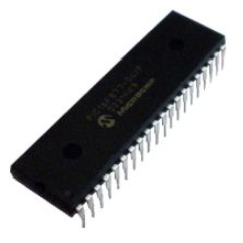
\includegraphics[scale=1]{images/pic.png}
	\caption{PIC18F452}	
	\label{fig:pic}	
\end{figure}

\newpage 
\section{Estrutura Interna}
A Figura \ref{fig:estuturapic} ilustra como é a estrutura interna do microcontrolador:

\begin{figure}[htp]
	\centering
	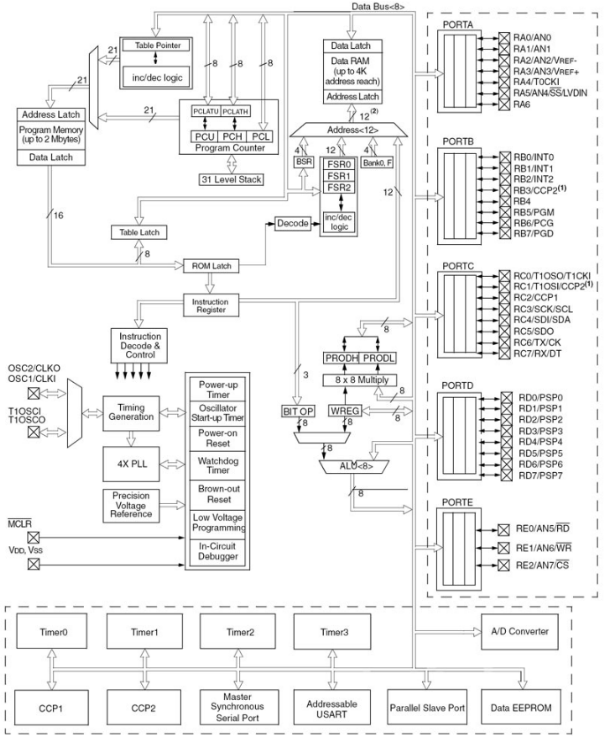
\includegraphics[scale=0.6]{images/estrutura_pic.png}
	\caption{Estrutura Interna PIC18F452}	
	\label{fig:estuturapic}	
\end{figure}

\newpage 
\section{DESCRIÇÃO DOS PINOS}
Dos 40 pinos desse microcontrolador 34 são pinos I/O, entrada e saída, divididos em 5 "PORT". A Figura \ref{fig:pinospic} representa uma relação dos pinos do microcontrolador.

\begin{figure}[htp]
	\centering
	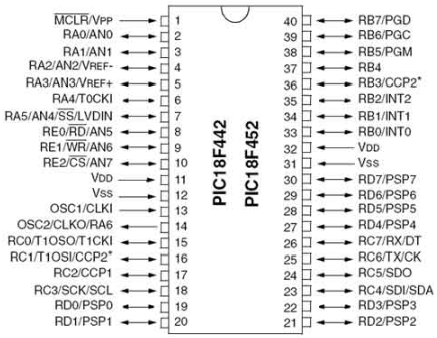
\includegraphics[scale=0.6]{images/pinos_pic.png}
	\caption{Pinos PIC18F452}	
	\label{fig:pinospic}	
\end{figure}

A divisão dos pinos I/O citada é da seguinte maneira:

\begin{itemize}
\item PORTA: São 7 pinos nomeados de RA0 a RA6. Podem ser utilizados como I/O geral ou conversor A/D, essa segundo opção tem exceção o pino RA4. Além de possuir a opção LVD, detecção de baixa tensão;
\item PORTB: São 8 pinos nomeados de RB0 a RB7. Podem ser utilizados para I/O geral e, além disso, pode-se trabalhar com três interrupções externas, módulo CCP, pinos de gravação e debug;
\item PORTC: São 8 pinos nomeados de RC0 a RC7. Podem ser utilizados para I/O geral, saída do oscilador do \emph{timer}, módulo CCP, Clock e data(dados) para os modos SPI, I2C e UART;
\item PORTD: São 8 pinos nomeados de RD0 a RD7. Podem ser utilizados para I/O geral ou como PSP para ter saída TTL, para interfaceamento com microprocessadores, por exemplo;
\item PORTE: São 3 pinos nomeados de RE0 a RE2. Podem ser utilizados para I/O geral ou pinos de controle de acesso.
\end{itemize}